\chapter{Resultados Parciais}\label{sec:resultados}
Neste capítulo os resultados parciais são apresentados divididos nas seguintes seções. A Seção \ref{sec:prova} destaca pontos relevantes de um artigo publicado no Simpósio Brasileiro de Informática na Educação (SBIE) responsável em nortear esta proposta. A Seção \ref{sec:reconhecedor} apresenta um estudo experimental comparativo sobre as arquiteturas de redes neurais de convolução relacionado ao domínio do problema e enquanto a Seção \ref{sec:considera} o resumo deste capítulo.   


\section{Prova de Conceito}\label{sec:prova}
Inicialmente, uma prova de conceito foi realizada para nortear o andamento deste projeto. O resultado desta prova de conceito foi publicada no Simpósio Brasileiro de Informática na Educação (SBIE) 2017 \citep{cruz2017framework}. Este trabalho consistiu na utilização da API da \textit{Microsoft Cognitives Services} um serviço na nuvem que oferece um conjunto de aplicações cognitivas, inclusive um reconhecedor de emoções via expressão facial. Esta experiência foi bastante positiva possibilitando ponderar as vantagens e desvantagens desta API, e assim, nortear a construção do reconhecedor de emoções proposto. A contribuição principal deste trabalho está em reconhecer emoções em tempo real, em um cenário real e de forma automática, com precisão aceitável em um ambiente educacional, correlacionando as emoções detectadas com o desempenho escolar em um teste. 

A revisão sistemática (ver Capítulo \ref{sec:revisaosistematica}) mostrou que os pesquisadores da área de reconhecimento de emoção ainda estão tímidos para colocar esses reconhecedores no mundo real. Desta forma, a utilização em cenários reais passa a ser um ponto de contribuição atestando que essas tecnologias estão amadurecendo possibilitando a integração a outros tipos de sistemas principalmente para tomadas de decisão, recomendações, análises de comportamento e entre outros. Contudo, funcionar no cenário real não é uma tarefa trivial, o reconhecedor deve alcançar uma excelente taxa de generalização, o mundo real é desafiador por haver muitas variações da face e do ambiente dificultando a precisão do algoritmo.  

\subsection{Síntese}
Neste artigo \citep{cruz2017framework}, propomos um \textit{framework} para detectar estados emocionais de alunos baseado em reconhecimento de expressões faciais no contexto das plataformas digitais educacionais. Analisamos e discutimos o uso de correlação e entropia entre os estados emocionais dos estudantes e o desempenho durante uma avaliação de múltipla escolha. Realizamos um experimento com 27 estudantes e elaboramos um teste composto de 40 perguntas. Na análise dos dados correlacionamos os estados emocionais de neutralidade, tristeza, felicidade, raiva, desgosto, medo, desprezo e surpresa detectados com o desempenho no teste. Concluímos que as questões que ocorreram maior variabilidade das emoções tinham também as maiores proporções de acertos.

\subsection{Objetivos}
O artigo \citep{cruz2017framework} tem como objetivo: (i) propor uma arquitetura de detecção automática de emoções para ambientes educacionais digitais por meio de reconhecimento automático de expressões faciais, utilizando processamento de imagens, de modo a tornar possível a obtenção de dados emocionais dos alunos durante o processo de aprendizagem, e (ii) analisar por meio de estatística descritiva um estudo de caso com dados obtidos a partir desta arquitetura. Esta análise pretende investigar e medir correlações entre as emoções e o desempenho obtido nas questões, levantando hipóteses relevantes sobre a relação entre os estados emocionais e o desempenho, o qual é relevante para sistemas de recomendações, tutores inteligentes e heurísticas em geral, que se interagem de forma dinâmica com as necessidades de aprendizado de cada aluno.

\subsection{Método Proposto}
A arquitetura proposta na Figura \ref{fig:metproposto} é formada pelos seguintes componentes: (i) uma plataforma educacional digital executada, por exemplo, em um \textit{tablet} com câmera frontal que possibilite a coleta de imagens das expressões faciais e das atividades dos alunos, relacionadas com a seleção das respostas e a navegação entre os diferentes objetos de aprendizagem; (ii) um classificador de emoções que recebe como entrada as imagens das expressões faciais e retorna um vetor com as probabilidades a posteriori das seguintes emoções: neutralidade, surpresa, felicidade, tristeza, desprezo, raiva, medo e desgosto; e (iii) um conjunto de métodos de estatística descritiva para realizar diversas análises úteis para: inferências, heurísticas, sistemas de recomendações, tutores inteligentes e inclusive para auxiliar o professor na tomada de decisões referentes às dificuldades de aprendizagem de cada aluno. A arquitetura proposta pode ser usada em tempo real, tanto em ambientes presenciais como à distância, possibilitando o cruzamento dos estados emocionais com a interação na plataforma.

\begin{figure}
\centering
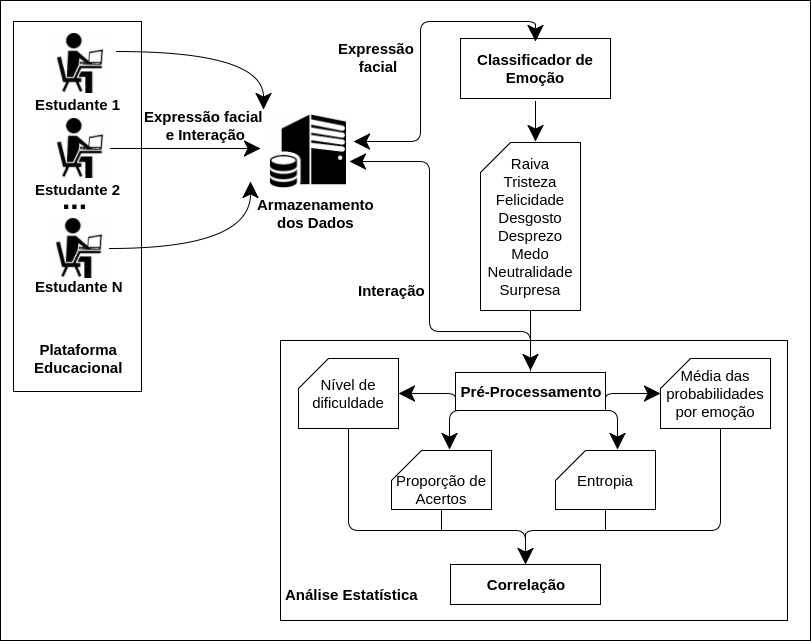
\includegraphics[scale=0.5]{figuras/diagrama.png}
\caption{Método Proposto}
\label{fig:metproposto}
\end{figure}

\subsubsection{Plataforma Educacional}
A plataforma educacional deve possuir um módulo coletor de dados que armazene continuamente os eventos da interação do estudante, tais como, a seleção das questões e suas respectivas respostas, e a identificação de todos os itens presentes na interface como botões, caixa de texto, opções de seleções e outros, assim como, a captura contínua da expressão facial do estudante.

Estes dados são armazenados para tornar possível diferentes análises, tais como: qual foi a emoção predominante na questão que os alunos mais erraram? Na questão que houve mais trocas de respostas qual foi a emoção predominante? Qual foi a emoção predominante no grupo de alunos que mais erraram as questões? Quais as emoções têm ocorrências na variação da dificuldade das questões? Isto pode ser um caminho para inferir a confusão via expressão facial que é um estado emocional não pertencente ao grupo das emoções básicas, entretanto, muito comum em ambiente educacional verificado por \cite{d2013beyond} que em alguns estudos de casos, concluíram que a confusão, tédio, curiosidade, engajamento, frustração e satisfação ocorrem cinco vezes mais do que as emoções básicas no âmbito educacional.

\subsubsection{Classificador de Emoção}
O classificador de emoção tem a função de identificar nas imagens as expressões faciais e atribuir um rótulo a cada imagem. Estes rótulos podem ser: neutralidade, raiva, felicidade, tristeza, desgosto, desprezo, medo e surpresa, como mencionado por \cite{ekman1994}, que são as emoções básicas capazes de ser reconhecidas dada uma expressão facial.

O classificador utilizado está descrito na Seção \ref{sec:plan}, e usufrui de técnicas de aprendizagem de máquina, mais especificamente de aprendizagem profunda em redes neurais pela arquitetura \textit{Convolutional Neural Network} (CNN), que tem sido o estado da
arte para este fim.

A saída do classificador de emoção para cada imagem recebida é um vetor de probabilidades que contém a probabilidade de cada emoção detectada na imagem \textit{i.e.: P=\{p\textsubscript{1},p\textsubscript{2},..,p\textsubscript{n}\}}, onde \textit{p\textsubscript{n}} representa a probabilidade a posteriori da detecção da n-ésima emoção. Uma propriedade é que a soma das probabilidades é igual a 1, e que a maior probabilidade presente no vetor corresponde ao rótulo final da emoção detectada na imagem, ou seja, a sua classificação \textit{e.g.: emoção = max(P)}.

\subsubsection{Análise Estatística}
Este componente contém outros subcomponentes que realizam análises acerca do desempenho e das emoções do estudante por meio da correlação de Pearson. Todos os subcomponentes recebem como entrada tanto os cliques de interação do estudante com a plataforma, como as classificações das expressões faciais. Desta forma, são recuperadas todas as instâncias necessárias para a realização do cruzamento da interação da plataforma com a emoção detectada, a fim de obter o coeficiente de correlação.

Um pré-processamento dos dados é executado antes da análise, onde é organizada a coleção de dados por questão, isto é, a reunião de todas as instâncias de todos os alunos com respeito a uma determinada questão e, desta forma, são agrupados a interação com a plataforma e os dados das classificações de emoções por questão. O
pré-processamento produz as seguintes informações para cada questão:

\begin{itemize}
 \item a média das probabilidades para cada emoção, incluindo todos os alunos;
 \item o nível de dificuldade;
 \item a proporção de acertos, por exemplo, se a metade dos alunos acertaram, então a
proporção é 50\%; e
 \item a entropia das emoções, que mede a dispersão das probabilidades das emoções
detectadas, isto é, caso em uma questão haja várias emoções diferentes e estejam
distribuídas uniformemente, a entropia será maior.
\end{itemize}
Todos esses dados pré-processados entram no componente de análise estatística,
e a sua saída pode ser útil para traçar um perfil emocional do estudante e da turma
mediante as correlações identificadas.

\subsection{Metodologia Experimental}
Um experimento foi realizado com 27 alunos do Ensino Médio de uma escola de tempo integral que farão o Exame Nacional do Ensino Médio (ENEM) 2017. O experimento consistiu em um simulado do exame contendo 40 questões de múltipla escolha.

\subsubsection{Planejamento}\label{sec:plan}
Adotamos uma plataforma educacional que permite a execução de questionários de múltipla escolha, coleta de cliques efetuados pelo estudante, captura automática de foto via câmera frontal do dispositivo, seja por \textit{tablet}, \textit{smartphone} ou \textit{notebook}. Os assuntos escolhidos foram: matemática, língua portuguesa, química, raciocínio lógico, geografia e história. O simulado teve duração de duas horas e cada questão possuía dois níveis de dificuldade (fácil ou difícil), além de ter cinco respostas alternativas.

Para o componente classificador, selecionamos a API da \textit{Microsoft Cognitives Services}, justamente por classificar bem emoções como neutralidade, felicidade e tristeza. Acreditamos que, no contexto da educação, uma emoção bastante comum é a neutralidade, pelo fato da expressão facial do estado de concentração se assemelhar bastante com a expressão facial de neutralidade reconhecida por esta API. Constatamos que estudantes quando estão pensando, estão concentrados, emitindo poucas movimentações intensas e variações de suas expressões faciais, assemelhando-se com a expressão de neutralidade.

\subsubsection{Execução}
A seleção dos estudantes para participar do experimento ocorreu voluntariamente. O grupo final formado foi heterogêneo, onde 53\% consideravam até o momento seu desempenho na escola como bom ou ótimo e, 47\% como regular ou ruim; além disso, 30\% deles consideravam a sua preparação para o vestibular como boa ou ótima e, 70\% como regular ou fraca. Os alunos selecionados são de turmas diferentes.

\subsection{Resultados e Discussões}
Inicialmente, obtemos os seguintes atributos calculados como os valores médios por questão, utilizando os dados coletados dos vinte e sete alunos: (i) a proporção de acertos; (ii) o nível de dificuldade; (iii) a média das probabilidades para cada emoção detectada; e (iv) a entropia por questão. Assim, obtemos um total de onze atributos (resumidos na Tabela \ref{tabelaArti}), onde cada um deles é representado por uma variável aleatória com quarenta valores.

Posteriormente, aplicamos a correlação de Pearson para analisar se há qualquer grau de correlação entre os pares dos atributos mencionados. A Tabela \ref{tabelaArti} apresenta a correlação entre a média das probabilidades de cada emoção com o nível de dificuldade e a proporção de acertos. Os principais resultados estão destacados em negrito.

Como podemos verificar na Tabela \ref{tabelaArti}, a expressão facial neutra possui uma correlação negativa com a proporção de acertos dos alunos (segunda coluna da Tabela \ref{tabelaArti}). Isto indica que estimular emoções diferentes da neutralidade durante a avaliação favorece o desempenho dos alunos. Um segundo indicativo de que isto ocorre, é dado pela correlação positiva entre o desprezo e a felicidade com a proporção de acertos e, de forma discreta, também ocorre com tristeza, surpresa e medo.

A entropia é calculada a partir do valor das probabilidades das emoções detectadas. Logo, percebemos que quando a neutralidade baixa, a entropia aumenta, o que significa que outras emoções estão sendo detectadas com maior probabilidade, ocorrendo a dispersão dos estados emocionais. Portanto, o fato de existir uma correlação positiva entre o aumento da entropia e a proporção de acertos reforça a observação constatada no parágrafo anterior. Adicionalmente, descobrimos que a emoção mais frequente foi a neutralidade, devido aos alunos passarem a maior parte do tempo concentrados analisando as questões para a busca de soluções. Assim, quando o nível de dificuldade da questão aumenta, a neutralidade também aumenta, isto pode ser um indício de que questões mais difíceis tem tendências de exigir maiores níveis de concentração do estudante.

Podemos considerar a hipótese de que, quando o estudante está respondendo uma questão, ao selecionar uma resposta, o mesmo tem uma percepção se acertou ou errou e, nesse momento, há possibilidade de emitir emoções positivas como felicidade e surpresa, ou emoções negativas como tristeza ou desprezo. Portanto, há uma variação dos estados emocionais durante o tempo de resposta de cada questão que deve ser considerado como um problema de mudança de estados. Este resultado é reforçado por
questões que ocasionaram maior entropia, ou seja, quanto maior a dispersão das emoções, maior é o índice de proporções de acertos.

A emoção desprezo aumenta a medida que as questões têm maiores proporções de acertos, isto pode ser explicado, pela mudança de estados durante o tempo de resposta de cada questão ou pelo fato da expressão facial de desprezo se assemelhar com a expressão facial de felicidade. Neste caso, é bem provável estar ocorrendo confusão por parte do classificador em diferenciar felicidade e desprezo.

\begin{table}[]\footnotesize
\centering
\caption{Resultado​ ​da​ ​correla\c{c}\~ao​ ​de​ ​Pearson​ ​para​ ​cada​ ​emo\c{c}\~ao​ ​detectada
e​ ​a​ ​entropia​ ​contra​ ​os​ ​atributos​ ​das​ ​quest\~oes}
\label{tabelaArti}
\begin{tabular}{|c|c|c|}
\hline
                      & \textbf{Nível de Dificuldade} & \textbf{Proporção de Acertos} \\ \hline
\textbf{Tristeza}     & \textbf{-0.33}                & 0.27                          \\ \hline
\textbf{Neutralidade} & \textbf{0.36}                 & \textbf{-0.48}                \\ \hline
\textbf{Desprezo}     & -0.15                         & \textbf{0.30}                 \\ \hline
Desgosto              & -0.13                         & 0.07                          \\ \hline
Raiva                 & -0.14                         & -0.08                         \\ \hline
Surpresa              & 0.07                          & 0.24                          \\ \hline
Medo                  & -0.06                         & 0.14                          \\ \hline
\textbf{Felicidade}   & -0.14                         & \textbf{0.31}                 \\ \hline
\textbf{Entropia}     & -0.12                         & \textbf{0.36}                 \\ \hline
\end{tabular}
\end{table}


Tanto a arquitetura para o reconhecimento de estados emocionais, como a
realização de análises de estados emocionais de estudantes, são úteis para a implementação de tutores inteligentes e sistemas de recomendações que possam fornecer personalização mais precisa do conteúdo para cada aluno levando em consideração seus estados emocionais. É importante identificar os casos diferentes da expressão neutra, justamente por serem menos frequentes podendo indicar alguma oportunidade de um tutor inteligente atuar.

Como trabalho futuro, pretendemos investigar a mudança temporal dos estados emocionais do estudante, mediante a estímulos produzidos por diferentes objetos de aprendizagem durante uma aula. Também, a implementação de uma heurística que considera o estado emocional do estudante para fornecer ajuda sob demanda com a intenção de aumentar o engajamento e o desempenho durante uma aula.

Finalmente, percebe-se que o \textit{framework} para classificação automática de emoções a partir de imagens necessita de um maior volume de dados, para reduzir eventuais erros de classificação, e permitir a classificação de novos tipos de emoções. Portanto, está nos nossos planos investigar alternativas para amenizar erros de classificação e melhorar a acurácia do \textit{framework}.

\section{Avaliação Experimental}\label{sec:avalexp}
% Base de dados
% Metodologia de Treinamento
% SW, HW, Setup
% Abordagem
% Arquiteturas de Redes Neurais
% Avaliação

Um estudo experimental foi realizado a fim de comparar diversos tipos de arquiteutras de redes neurais de convolução. Este estudo tem como objetivo eleger a arquitetura que gerou o melhor modelo avaliando a precisão, revocação e acurácia.  


Foi iniciado o desenvolvimento do reconhecedor de emoção, visto que, para trabalhar com redes profundas, especificamente com as redes neurais de convolução é necessário dispor de grandes quantidades de recursos computacionais relacionadas a memória e a processamento. Por isso, como ponto de partida optamos por uma arquitetura reduzida da AlexNet ilustrada na Figura \ref{fig:implementadaarquitetura}, utilizamos esta arquitetura para treinar e gerar um modelo para classificar emoções em expressões faciais.

Para gerar o modelo utilizamos a base de dados \textit{FER-2013} tanto para treinar como para validar, esta base é bastante utilizada pela literatura e contém 28709 imagens de expressão facial com as seguintes emoções (classes): raiva, desgosto, medo, felicidade, tristeza, surpresa e neutralidade. Foi utilizado 2/3 da base de dados para treinamento e o restante para validação. A rede foi treinada por 140 épocas e alcançou os seguintes resultados expresso na matriz de confusão na Figura \ref{fig:confusionmatrix}. Para implementação da rede neural de convolução foi utilizado o \textit{framework Tensorflow} (\url{https://www.tensorflow.org/}), em um computador com a seguinte configuração: \textit{GPU NVIDIA GEFORCE 930}, \textit{Intel Core-i7} e \textit{16 GB de RAM DDR4}. 

Seguimos a abordagem proposta na Seção \ref{sec:abordagemproposta}, e como detector de face utilizamos o Viola Jones implementado pela biblioteca \textit{OpenCV 3.0} (\url{https://opencv-python-tutroals.readthedocs.io/en/latest/}), nesta implementação diferentemente da abordagem proposta, foi realizado uma normalização transformando a imagem em escala de cinza (ver Figura \ref{fig:implementadaarquitetura}). Esta implementação foi anteriormente a revisão sistemática da literatura, a revisão mostrou que as redes neurais de convolução sabem lidar com a imagem colorida, então, é desnecessário transformar em escala de cinza, no entanto, pode ser interessante em uma configuração de experimento verificar qual a melhor proposta com a imagem colorida ou em escala de cinza. 

\begin{figure}
\centering
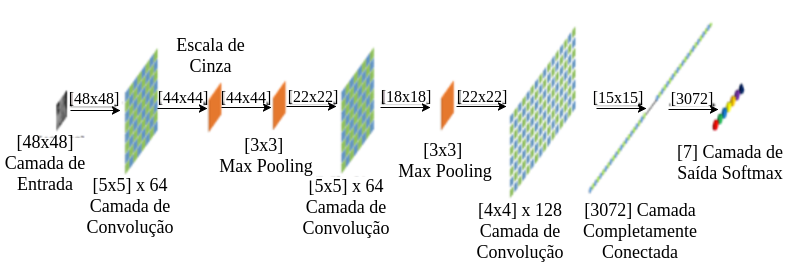
\includegraphics[scale=0.57]{figuras/arquiteturaimplementada.png}
\caption{Arquitetura Implementada de Rede Neural de Convolução}
\label{fig:implementadaarquitetura}
\end{figure}


\begin{figure}
\centering
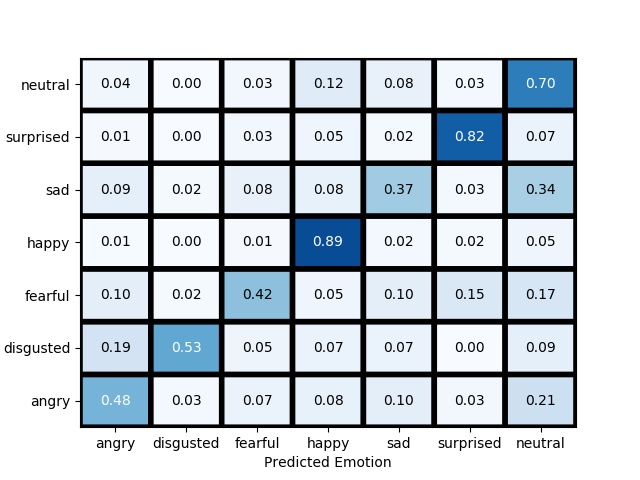
\includegraphics[scale=0.8]{figuras/confusion-matrix-75split-140epo.png}
\caption{Matriz de Confusão com 140 épocas de treinamento}
\label{fig:confusionmatrix}
\end{figure}

\section{Resumo}\label{sec:considera}
Foi possível verificar que o reconhecedor de emoção tem muita aplicação, iniciamos nossa aplicação no cenário real em uma prova de conceito na área de educação, no qual há muitas utilidades. Esta prova de conceito nos deu norte para a evolução desta proposta. Consequentemente foi iniciado o desenvolvimento do reconhecedor que esta proposta pretende gerar como contribuição. Há muitos trabalhos futuros, principalmente combinar as diversas técnicas de pré-processamento com as diversas arquiteturas de RNC juntamente com as bases de dados. A área de aprendizagem de máquina costuma ser bastante experimental e aparentemente temos bastante configuração de experimento para testar, até encontrar a melhor taxa de aprendizado da RNC.


% Please add the following required packages to your document preamble:
% \usepackage{multirow}
\begin{table}[]
\centering
\caption{Resultados experimentais de redes neurais convolução}
\label{my-label}
\begin{tabular}{llcccc}
\hline
\textbf{Arquitetura}                & \textbf{Emoção}       & \textbf{Precisão} & \textbf{Revocação} & \textbf{F1-score} & \textbf{Acurácia}               \\ \hline
\multirow{8}{*}{Alexnet}            & Raiva                 & 0.51              & 0.60               & 0.55              & \multirow{8}{*}{0.712}          \\
                                    & Desgosto              & 0.62              & 0.64               & 0.63              &                                 \\
                                    & Medo                  & 0.47              & 0.41               & 0.44              &                                 \\
                                    & Felicidade            & 0.84              & 0.89               & 0.86              &                                 \\
                                    & Tristeza              & 0.64              & 0.50               & 0.56              &                                 \\
                                    & Surpresa              & 0.84              & 0.77               & 0.80              &                                 \\
                                    & Neutralidade          & 0.62              & 0.64               & 0.63              &                                 \\
                                    & Média/Total           & 0.71              & 0.71               & 0.71              &                                 \\ \hline
\multirow{8}{*}{Inception-V3}       & Raiva                 & 0.54              & 0.51               & 0.52              & \multirow{8}{*}{0.701}          \\
                                    & Desgosto              & 0.56              & 0.57               & 0.56              &                                 \\
                                    & Medo                  & 0.47              & 0.42               & 0.44              &                                 \\
                                    & Felicidade            & 0.88              & 0.88               & 0.88              &                                 \\
                                    & Tristeza              & 0.47              & 0.53               & 0.50              &                                 \\
                                    & Surpresa              & 0.85              & 0.79               & 0.82              &                                 \\
                                    & Neutralidade          & 0.59              & 0.62               & 0.61              &                                 \\
                                    & Média/Total           & 0.70              & 0.70               & 0.70              &                                 \\ \hline
\multirow{8}{*}{\textbf{Resnet-32}} & \textbf{Raiva}        & \textbf{0.69}     & \textbf{0.57}      & \textbf{0.62}     & \multirow{8}{*}{\textbf{0.757}} \\
                                    & \textbf{Desgosto}     & \textbf{0.79}     & \textbf{0.66}      & \textbf{0.72}     &                                 \\
                                    & \textbf{Medo}         & \textbf{0.45}     & \textbf{0.50}      & \textbf{0.47}     &                                 \\
                                    & \textbf{Felicidade}   & \textbf{0.90}     & \textbf{0.89}      & \textbf{0.90}     &                                 \\
                                    & \textbf{Tristeza}     & \textbf{0.60}     & \textbf{0.65}      & \textbf{0.63}     &                                 \\
                                    & \textbf{Surpresa}     & \textbf{0.82}     & \textbf{0.86}      & \textbf{0.84}     &                                 \\
                                    & \textbf{Neutralidade} & \textbf{0.67}     & \textbf{0.68}      & \textbf{0.68}     &                                 \\
                                    & \textbf{Média/Total}  & \textbf{0.76}     & \textbf{0.76}      & \textbf{0.76}     &                                 \\ \hline
\end{tabular}
\end{table}